\RCS$Revision: 423381 $
\RCS$HeadURL: svn+ssh://svn.cern.ch/reps/tdr2/papers/HIN-16-011/trunk/HIN-16-011.tex $
\RCS$Id: HIN-16-011.tex 423381 2017-09-01 14:20:05Z alverson $
\newlength\cmsFigWidth
\ifthenelse{\boolean{cms@external}}{\setlength\cmsFigWidth{0.98\columnwidth}}{\setlength\cmsFigWidth{0.69\textwidth}}
\ifthenelse{\boolean{cms@external}}{\providecommand{\cmsLeft}{top\xspace}}{\providecommand{\cmsLeft}{left\xspace}}
\ifthenelse{\boolean{cms@external}}{\providecommand{\cmsRight}{bottom\xspace}}{\providecommand{\cmsRight}{right\xspace}}
\newcommand{\sqrts}{ \ensuremath{\sqrt{s}}\xspace}
\newcommand{\sqrtsNN}{ \ensuremath{\sqrt{\smash[b]{s_{_{\mathrm{NN}}}}}}\xspace}
\newcommand{\Bplusminusdecay}{\ensuremath{\PBpm\to\PJGy~\PKpm\to\Pgmp\Pgmm\PKpm}\xspace}
\newcommand{\Bjpsixdecay}{\ensuremath{\PB\to\PJGy~\cmsSymbolFace{X}}\xspace}
\newcommand{\RAA}{\ensuremath{R_{\mathrm{AA}}}\xspace}
\newcommand{\TAA}{\ensuremath{T_{\mathrm{AA}}}\xspace}
\newcommand{\pPb}{\ensuremath{\Pp\mathrm{Pb}}\xspace}
\newcommand{\PbPb}{\ensuremath{\mathrm{PbPb}}\xspace}
\newcommand{\Pb}{\ensuremath{\mathrm{Pb}}\xspace}
\newcommand{\pp}{\Pp\Pp\xspace}
\newcommand{\Bp}{ \ensuremath{\rm B^{+}}\xspace}
\newcommand{\Bsp}{ \ensuremath{\rm B_{\rm s }^{+}}\xspace}
\newcommand{\Dsp}{ \ensuremath{\rm D_{\rm s }^{+}}\xspace}
\newcommand{\Bspm}{ \ensuremath{\rm B_{\rm s }^{\pm}}\xspace}

\providecommand{\mbinv} {\mbox{\ensuremath{\,\text{mb}^\text{$-$1}}}\xspace}
\providecommand{\HYDJET}{\textsc{hydjet}\xspace}

\cmsNoteHeader{HIN-16-011}

\title{\texorpdfstring{Measurement of the $\Bsp$ meson nuclear modification factor in \PbPb collisions at $\sqrtsNN=5.02\TeV$}{Measurement of Bs+/- mesons nuclear modification factor in PbPb collisions at sqrt(s[NN]) = 5.02 TeV}}

\address[cern]{CERN}
\author[cern]{The CMS Collaboration}

\date{\today}

\abstract{
%The differential production cross sections of $\PBpm$ mesons are measured via the exclusive decay channels \Bplusminusdecay as a function of transverse momentum in \pp and \PbPb collisions at a center-of-mass energy $\sqrtsNN=5.02\TeV$ per nucleon pair with the CMS detector at the LHC.
%The \pp (\PbPb) dataset used for this analysis corresponds to an integrated luminosity of 28.0\pbinv (351\mubinv).
%The measurement is performed in the $\PBpm$ meson transverse momentum range of 7 to 50\GeVc, in the rapidity interval $\abs{y}<2.4$. In this kinematic range, a strong suppression of the production cross section by about a factor of two is observed in the \PbPb system in comparison to the expectation from \pp reference data. These results are found to be roughly compatible with theoretical calculations incorporating beauty quark diffusion and energy loss in a quark-gluon plasma.
}

\hypersetup{%
pdfauthor={Ta-Wei Wang, Andrew Turner, Jing Wang, Dozen Candan, Kisoo Lee, Gian Michele Innocenti, Hyunchul Kim, Camelia Mironov, Yen-Jie Lee},%
pdftitle={Measurement of B+/- meson differential production cross sections in pp and PbPb collisions at sqrt(s[NN]) = 5.02 TeV},%
pdfsubject={CMS},%
pdfkeywords={physics, dimuons, proton Lead, charmonia, suppression, quark gluon plasma, shadowing, B meson, open heavy-flavor}}

\maketitle

Relativistic heavy ion collisions allow the study of quantum chromodynamics (QCD) at high energy density and temperature. Under such extreme conditions, a state consisting of deconfined 
quarks and gluons, the quark-gluon plasma (QGP)~\cite{QGP1,QGP2}, is predicted by lattice QCD calculations~\cite{Karsch:2003jg}. Heavy-quarks are effective probes to study the 
properties of this medium. Charm and beauty quarks, which are produced in hard scatterings at the early stages of the collision, are expected to lose energy via elastic collisions and 
medium-induced gluon radiation. The study of this phenomenon, called jet quenching~\cite{Eloss1,Baier:2000mf,Chatrchyan:2011sx,Aad:2010bu}, can provide strong insights into the 
energy density and diffusion properties of the Quark-Gluon Plasma.  The measurement of the suppression of strange beauty particles in heavy-ion collisions is 
also considered of fundamental importance to study the mechanisms of beauty hadronisation in heavy ion collisions. In presence of a medium with increased strangeness content 
as the QGP~\cite{ABELEV:2013zaa}, the relative yield of $\Bspm$ mesons with respect to non-strange beauty mesons at low-intermediate \pt can be enhanced in nucleus-nucleus 
collisions as compared to pp interactions if recombination is a relevant mechanism of beauty hadronisation in the QGP~\cite{Molnar:2003ff,Greco:2003mm,Greco:2003vf}. 
An indication of the relevance of recombination, which is considered one of the golden probe to identify the presence of a deconfined medium, was recently observed in the charm sector by the ALICE 
Collaboration that measured an enhancement in the relative yield of $\Dsp$ mesons with respect to non-strange charmed mesons in central PbPb collisions at $\sqrts=5.02\TeV$~\cite{Adam2016Ds}.

The production of $\Bsp$ mesons was measured at the LHC in pp collisions at center-of-mass energies of $\sqrts=7\TeV$~\cite{Chatrchyan:2011vh}
and in in proton-lead (pPb) collisions at a center-of-mass energy per nucleon pair $\sqrts=5.02\TeV$~\cite{Khachatryan:2015uja}.
In this Letter, we perform the first measurement of exclusive $\Bspm$ mesons decays in PbPb collisions. The nuclear modification factor \RAA of $\Bp$ mesons, 
which is defined as the ratio of the cross section in PbPb collisions with respect to that in pp collisions scaled by the number of binary nucleon-nucleon (NN) collisions, 
is also presented. The comparison between the \RAA of $\Bsp$ and the one of $\Bp$ mesons, which was also recently measured by the CMS Collaboration~\cite{PhysRevLett.119.152301}, provides
important insights into the role of beauty recombination in heavy-ion collisions. 


\begin{figure*}[tb]
\centering
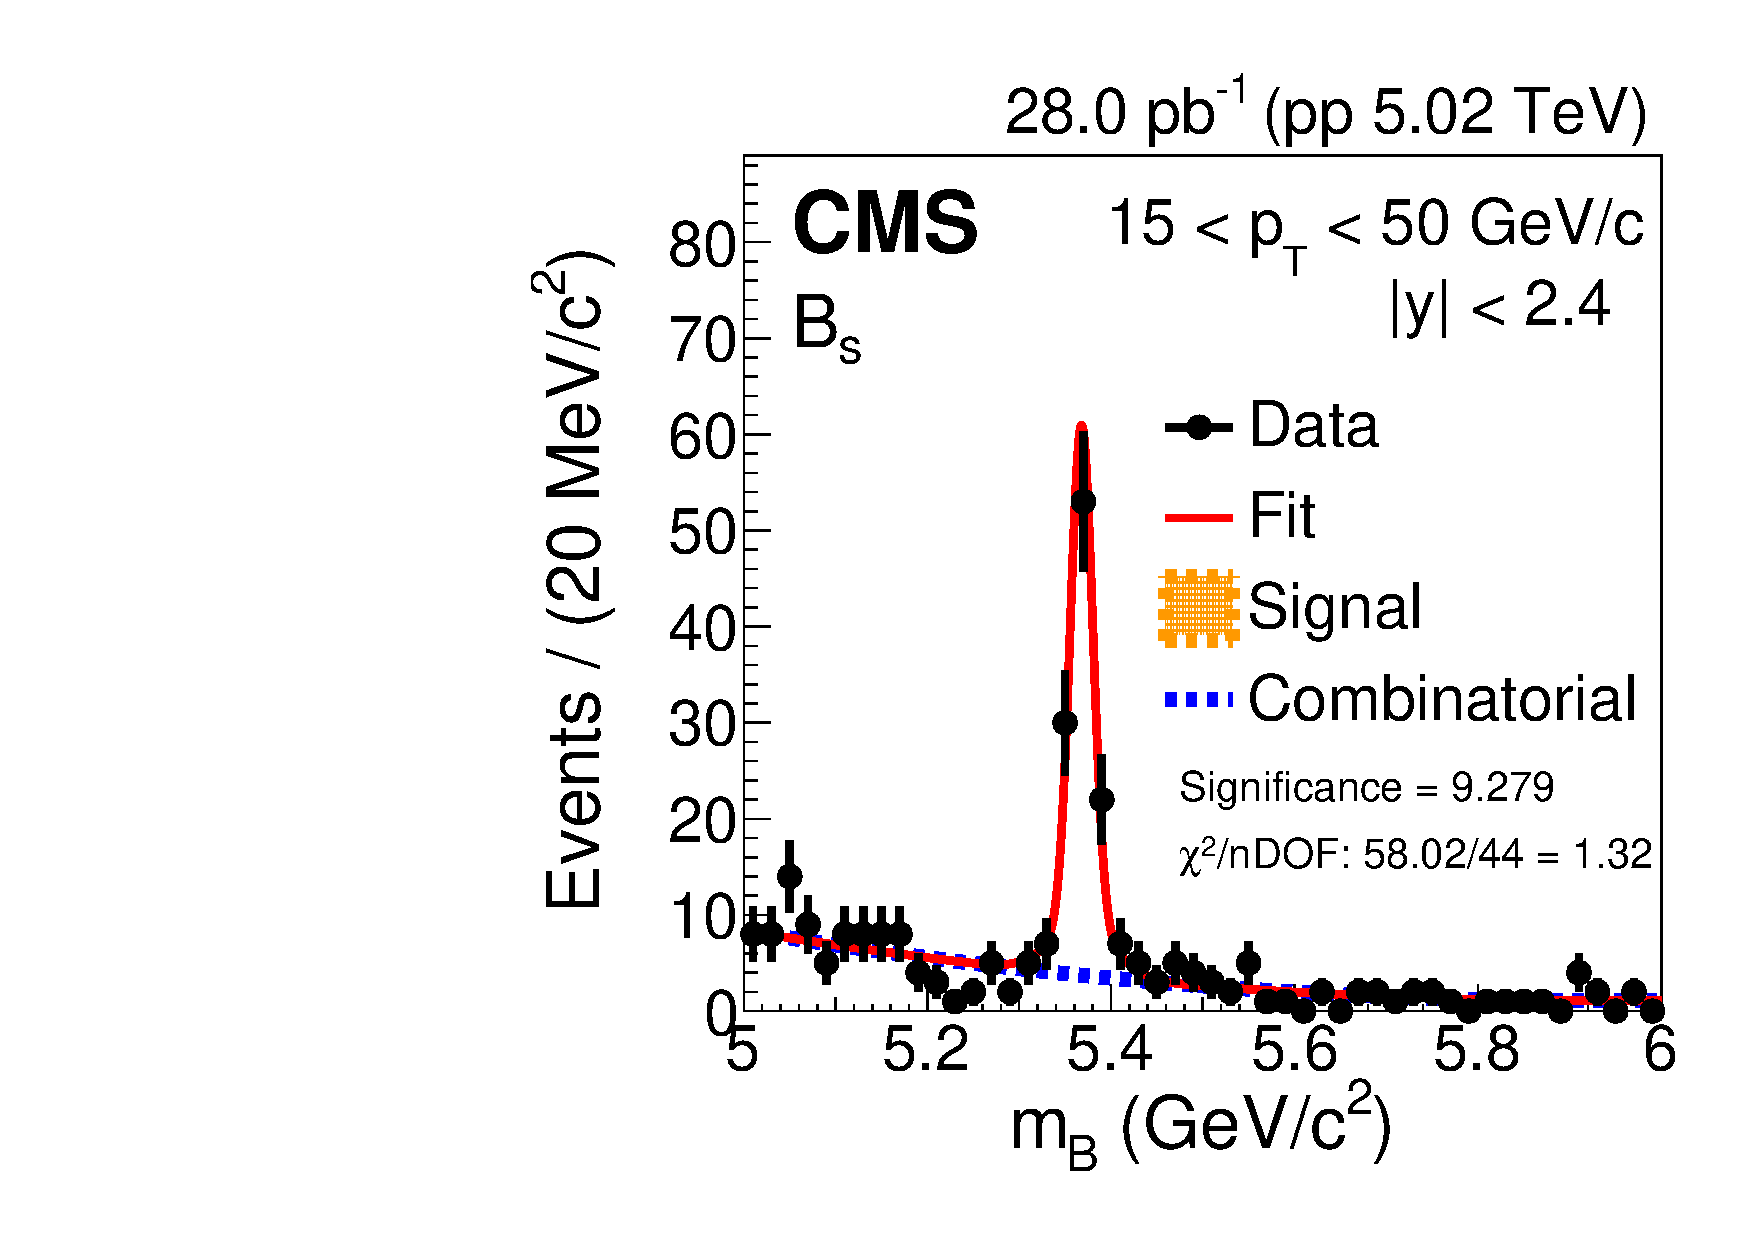
\includegraphics[width=.49\textwidth]{plots/data_pp_15_50.pdf}
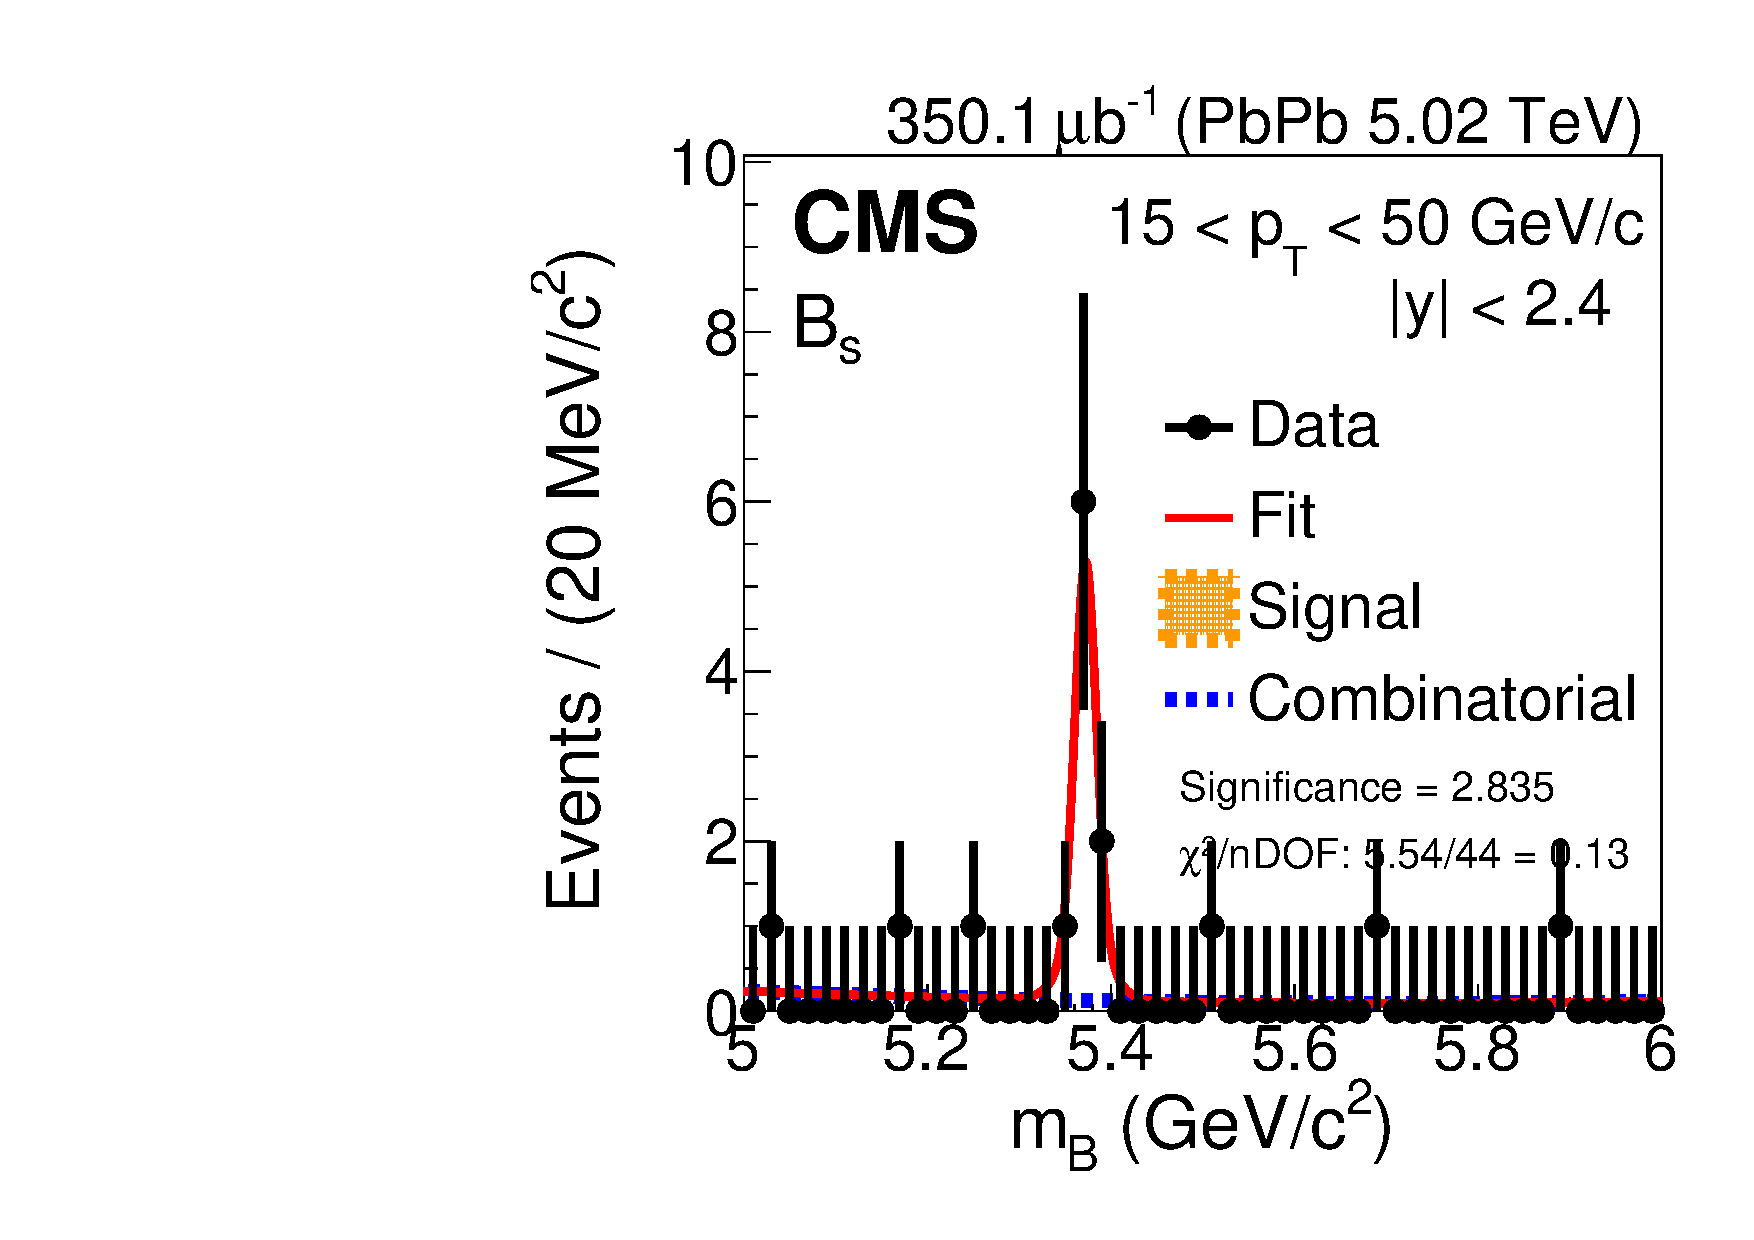
\includegraphics[width=.49\textwidth]{plots/data_PbPb_15_50.pdf}
\caption{Invariant mass distributions of $\Bspm$ candidates in \pp (left) and \PbPb (right) collisions measured in $\abs{y}<2.4$ and in the \pt region 15--50\GeVc.} 
\label{fig:rawYieldsBsmeson}
\end{figure*}

\begin{figure*}[tb]
\centering
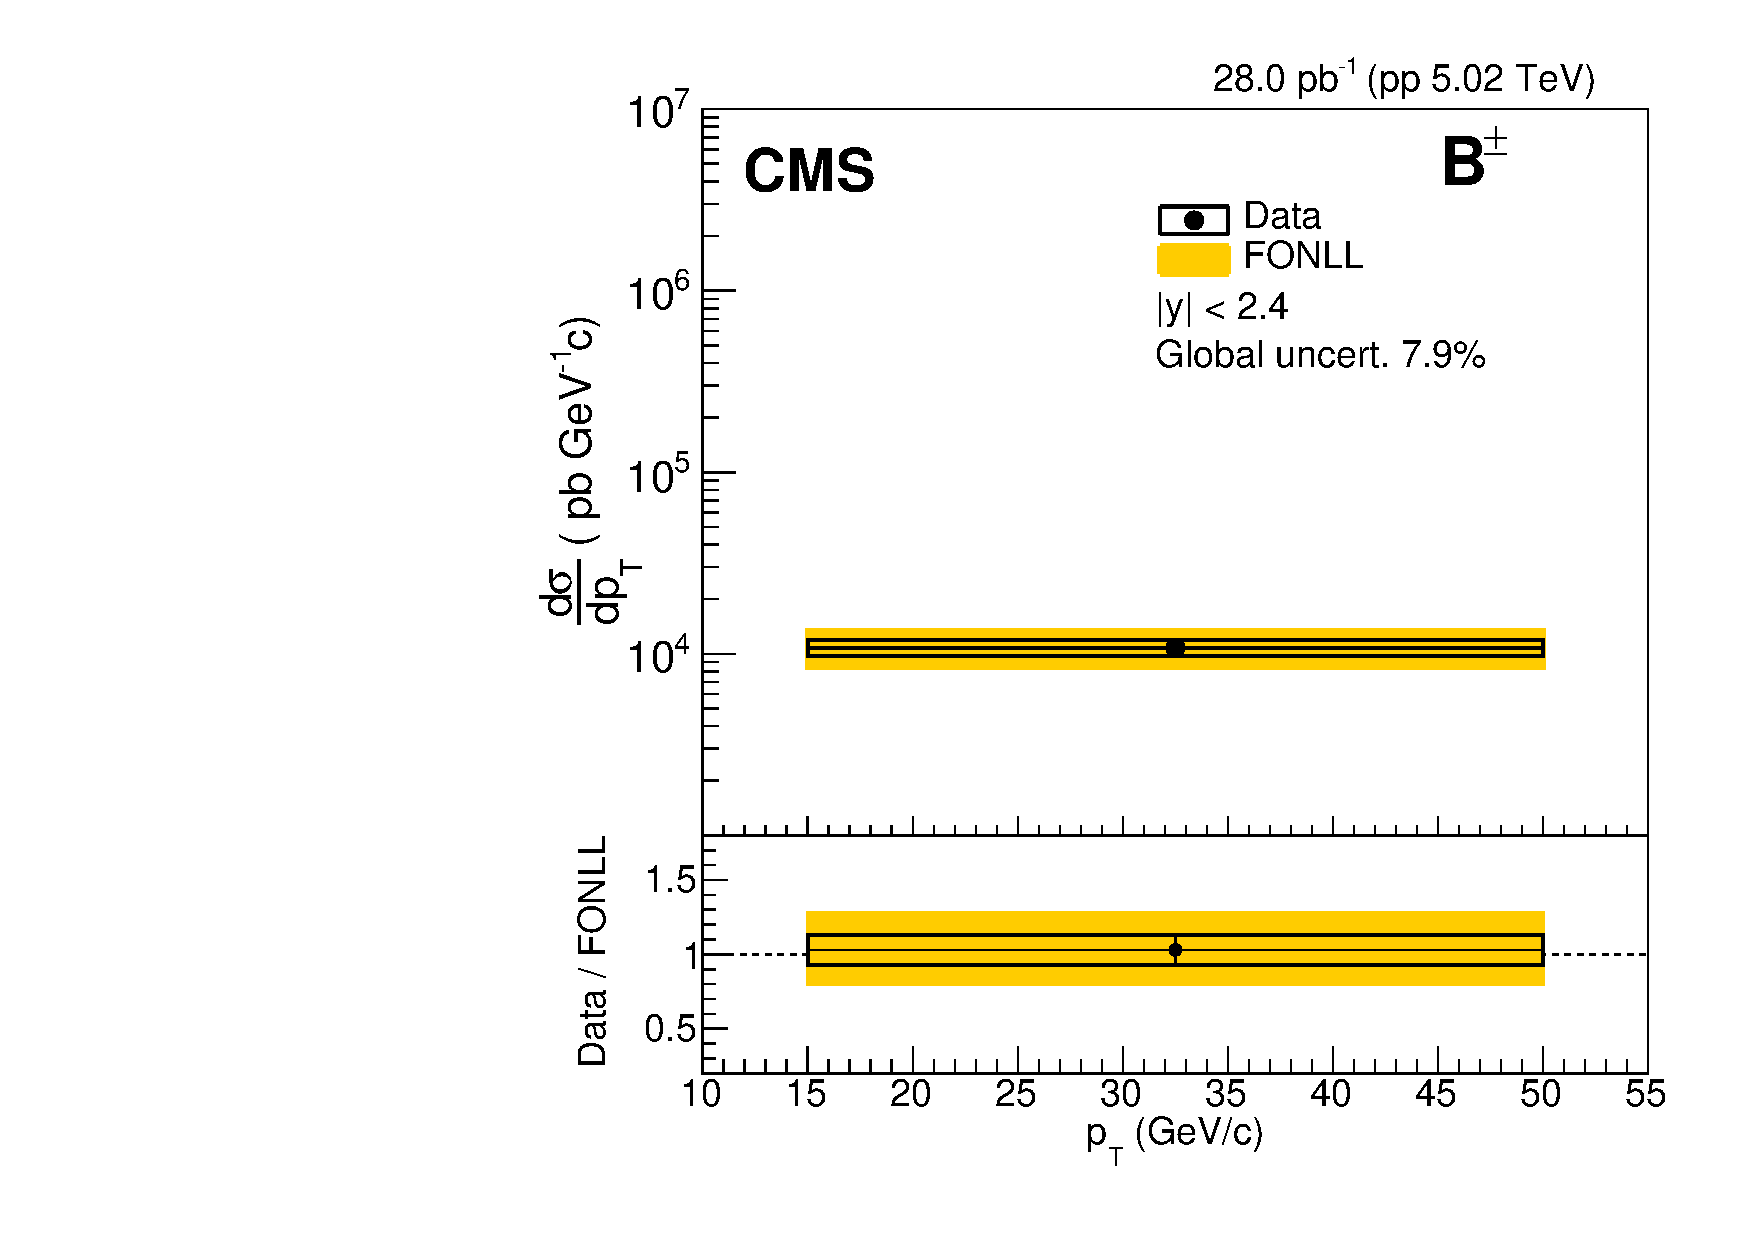
\includegraphics[width=.45\textwidth]{plots/canvasSigmaBplusRatiopp.pdf}
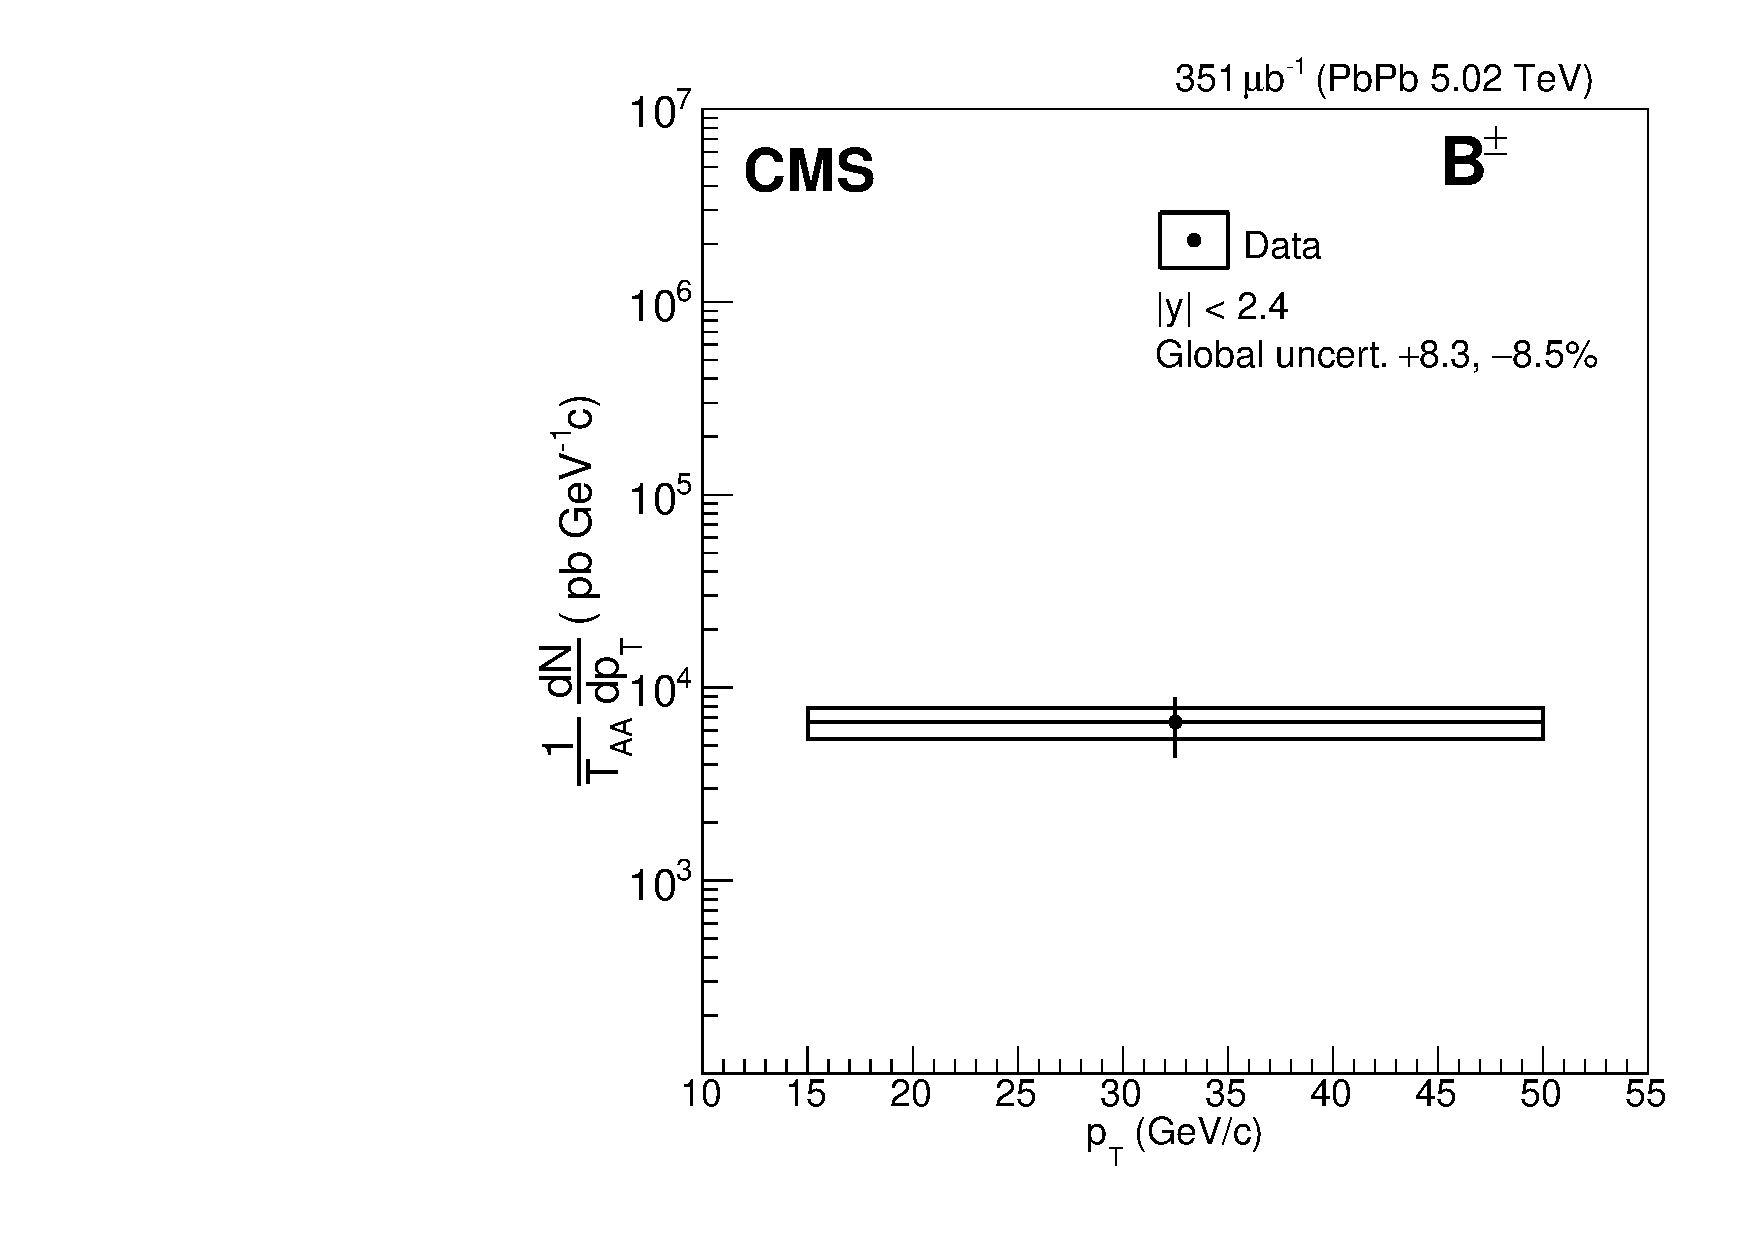
\includegraphics[width=.45\textwidth]{plots/canvasSigmaBplusRatioPbPb_0_100.pdf}
\caption{
The \pt-differential production cross section of $\Bsp$ in \pp (left) and \PbPb (right) collisions at $\sqrts=5.02\TeV$. The vertical bars (boxes) correspond to statistical (systematic) uncertainties.
The systematic uncertainty boxes here include both the correlated and uncorrelated contributions added in quadrature. The global systematic uncertainty, listed in the legend and not included in the point-to-point uncertainties. 
For the \pp cross section, they comprise the uncertainties in the integrated luminosity measurement and in the branching fraction $\mathcal{B}$. For the \PbPb cross section, they comprise the uncertainties in \TAA, $N_{\text{MB}}$, and $\mathcal{B}$.
The \pp cross section is compared to FONLL calculations~\cite{FONLLcharmbottomPP1,FONLLcharmbottomPP2,FONLLcharmbottomPP3} represented by the colored boxes with the heights indicating the theoretical uncertainty.}
\label{fig:crosssections}
\end{figure*}


\begin{figure}[tb]
\centering
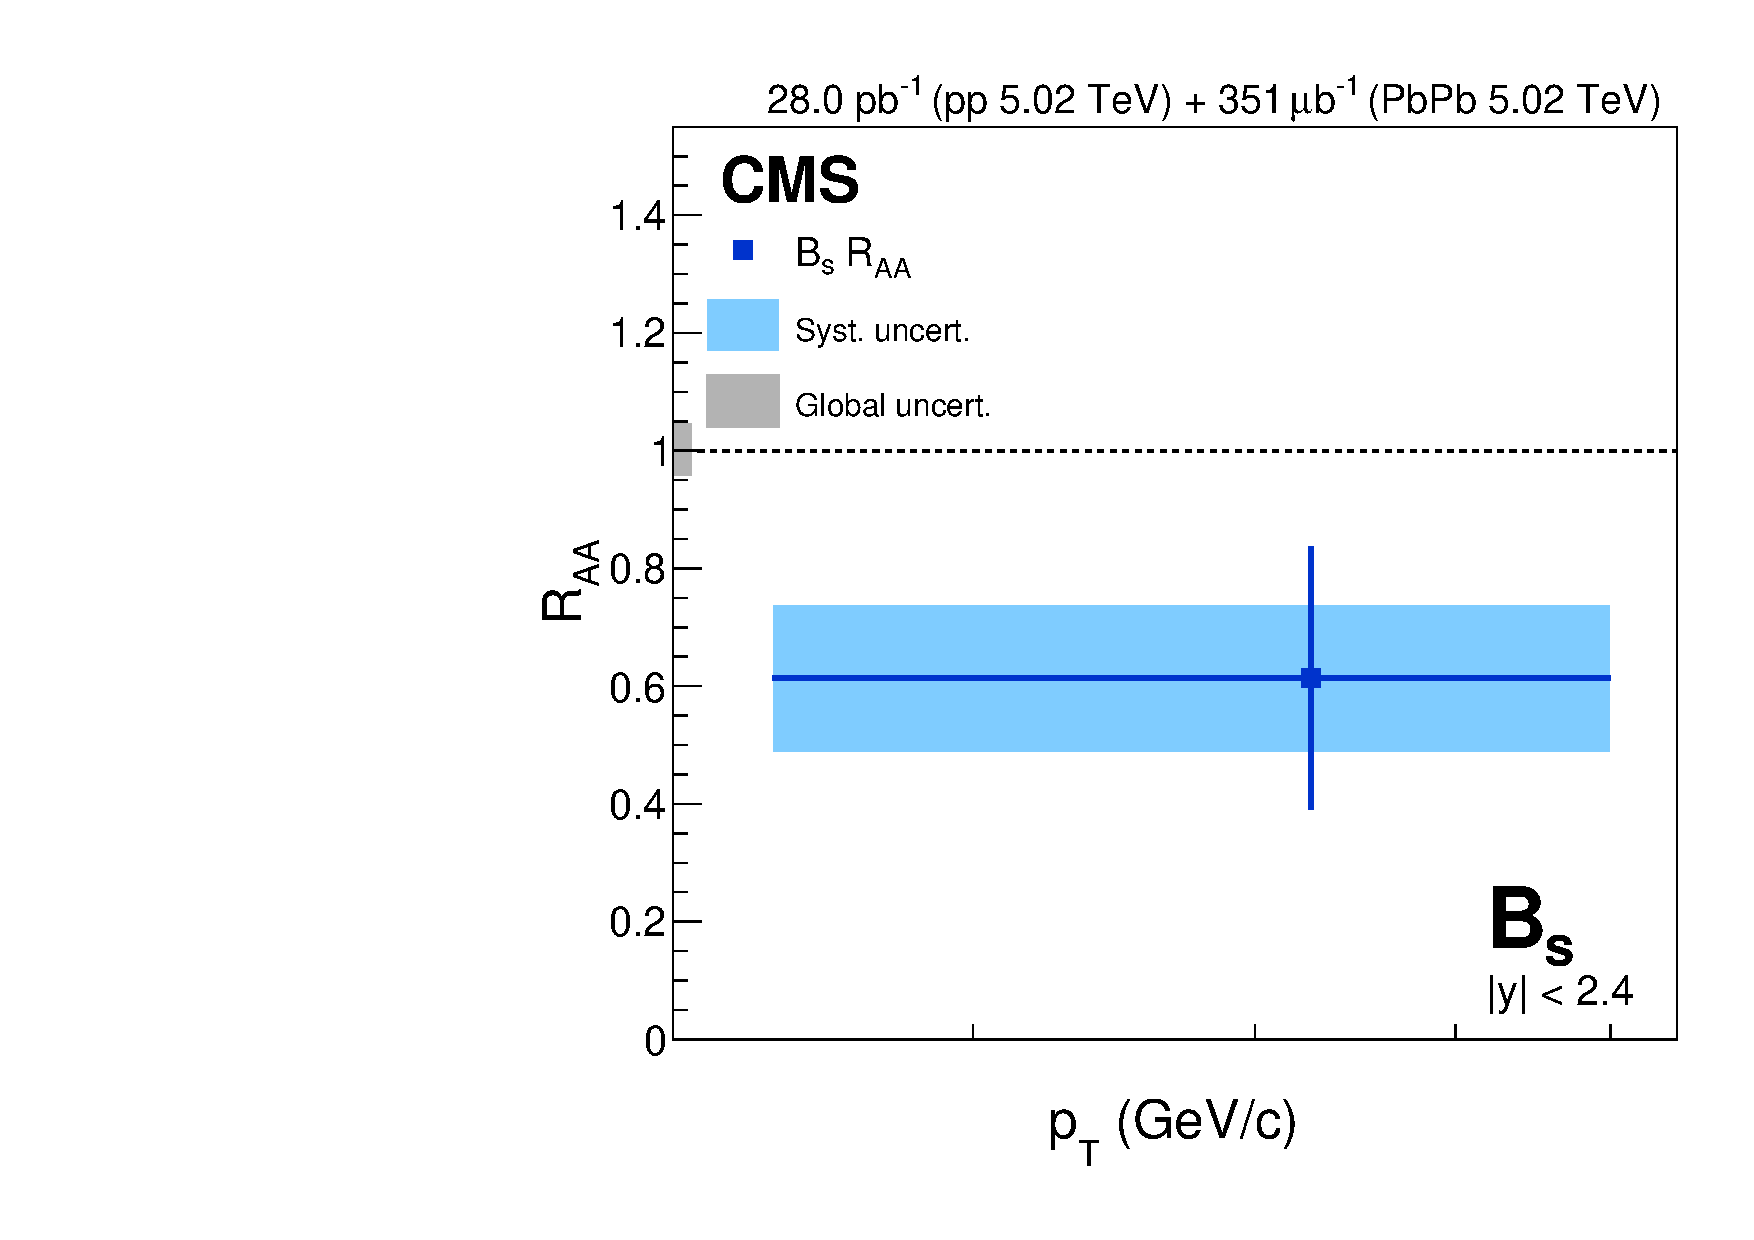
\includegraphics[width=\cmsFigWidth]{plots/canvasRAAPbPb_0_100.pdf}
\caption{The \pt dependence of the nuclear modification factor \RAA of $\Bsp$ measured in \PbPb collisions at $\sqrtsNN=5.02\TeV$. The vertical bars (boxes) correspond to statistical (systematic) uncertainties.
The global systematic uncertainty, represented as a grey box at $\RAA=1$, comprises the uncertainties in the integrated luminosity measurement and \TAA value. }
%Four theoretical calculations are also shown for comparison: TAMU~\cite{He:2011qa, He:2014cla}, Djordjevic~\cite{Djordjevic:2016vfo}, CUJET3.0~\cite{Xu:2015bbz, Xu:2014tda, Xu:2014ica}, and AdS/CFT HH~\cite{Horowitz:2015dta,  AdscftHH}. The line width of the theoretical calculation from Ref.~\cite{He:2011qa, He:2014cla} represents the size of its statistical uncertainty.}
\label{fig:rpaall}
\end{figure}


\begin{acknowledgments}
We congratulate our colleagues in the CERN accelerator departments for the excellent performance of the LHC and thank the technical and administrative staffs at CERN and at other CMS institutes for their contributions to the success of the CMS effort. In addition, we gratefully acknowledge the computing centers and personnel of the Worldwide LHC Computing Grid for delivering so effectively the computing infrastructure essential to our analyses. Finally, we acknowledge the enduring support for the construction and operation of the LHC and the CMS detector provided by the following funding agencies: BMWFW and FWF (Austria); FNRS and FWO (Belgium); CNPq, CAPES, FAPERJ, and FAPESP (Brazil); MES (Bulgaria); CERN; CAS, MoST, and NSFC (China); COLCIENCIAS (Colombia); MSES and CSF (Croatia); RPF (Cyprus); SENESCYT (Ecuador); MoER, ERC IUT, and ERDF (Estonia); Academy of Finland, MEC, and HIP (Finland); CEA and CNRS/IN2P3 (France); BMBF, DFG, and HGF (Germany); GSRT (Greece); OTKA and NIH (Hungary); DAE and DST (India); IPM (Iran); SFI (Ireland); INFN (Italy); MSIP and NRF (Republic of Korea); LAS (Lithuania); MOE and UM (Malaysia); BUAP, CINVESTAV, CONACYT, LNS, SEP, and UASLP-FAI (Mexico); MBIE (New Zealand); PAEC (Pakistan); MSHE and NSC (Poland); FCT (Portugal); JINR (Dubna); MON, RosAtom, RAS, RFBR and RAEP (Russia); MESTD (Serbia); SEIDI, CPAN, PCTI and FEDER (Spain); Swiss Funding Agencies (Switzerland); MST (Taipei); ThEPCenter, IPST, STAR, and NSTDA (Thailand); TUBITAK and TAEK (Turkey); NASU and SFFR (Ukraine); STFC (United Kingdom); DOE and NSF (USA).
\end{acknowledgments}

\bibliography{auto_generated}



